%%%%%%%%%%%%%%%%%%%%%%%%%%%%%%%%%%%%%%
% One Column
%%%%%%%%%%%%%%%%%%%%%%%%%%%%%%%%%%%%%%
\documentclass[smallabstract,smallcaptions]{dccpaper}

\usepackage{epsfig}
\usepackage{epstopdf}
\usepackage{cite}
\usepackage{amsmath}
\usepackage{amssymb}
\usepackage{color}
\usepackage{url}

\newlength{\figurewidth}
\newlength{\smallfigurewidth}


%%%%%%%%%%%%%%%%%%%%%%%%%%%%%%%%%%%%%%
% One Column
%%%%%%%%%%%%%%%%%%%%%%%%%%%%%%%%%%%%%%
\setlength{\smallfigurewidth}{2.75in}
\setlength{\figurewidth}{6in}

\begin{document}

\title
{\large
\textbf{Universal Rate-Distortion Analysis for Various Source Distributions}
}

\author{%
Shengbin Meng, Jun Sun$^{\ast}$, Yizhou Duan, and Zongming Guo\\[0.5em]
{\small\begin{minipage}{\linewidth}\begin{center}
\begin{tabular}{ccc}
Institution of Computer Science and Technology, \\
Peking University, Beijing, 100086, China\\
\url{{mengshengbin, sunjun, duanyizhou, guozongming}@pku.edu.cn}
\end{tabular}
\end{center}\end{minipage}}
}

\maketitle
\thispagestyle{empty}

\begin{abstract}
This paper studies the complex rate-distortion (R-D) analysis problem from a universal perspective. First, it is revealed that, for any source distribution composed of a scaling factor (SF) and the remaining part, SF does not affect the derivative of its R-D function (with PSNR as distortion criteria). This universal property can properly reduce the complexity of R-D modeling for real sources. Second, universal principles for the widely-used quantization scheme to achieve optimum R-D performance are deduced regardless of the source distribution form, which can be utilized to conveniently guide the practical quantizer design. Simulation experiments for Cauchy distribution, which still lacks thorough analysis in the literature, are presented to validate the universal property and principles.
\end{abstract}

\section{Introduction}

\let\thefootnote\relax\footnotetext{* is the corresponding author.}

As one of the fundamental issues of source coding, rate-distortion (R-D) analysis has attracted considerable research attention. In general, R-D analysis focuses on studying the essential relationship between rate and distortion of the source under applicable quantization technologies. A source is typically characterized by its probability distribution, while the transform-based entropy-constrained scalar quantization is the most extensively applied quantization technology \cite{Hang_TCSVT1997}. Therefore, R-D analysis is usually represented by studying the R-D relationship and R-D performance of applying certain scalar quantizer to a given source distribution.

On one hand, to evaluate the best attainable R-D performance, different types of scalar quantizers were analyzed and compared \cite{Sullivan_TIT1996}, among which the dead-zone plus uniform threshold quantizer (DZ+UTQ) with nearly-uniform reconstruction quantizer (NURQ) is recommended and now applied in all major international coding standards \cite{Sullivan_VCIP2005}. On the other hand, regarding to which distribution is most appropriate to statistically characterize the source in real compression applications, no consensus is ever reached. Take the DCT coefficients encountered in image/video coding for example. Some researchers prefer to describe that with Gaussian, Laplacian, or their parametric family generalized Gaussian distribution (GGD) \cite{Pratt_Wiley1978,Smooth_SPIE1996,Sun_TCSVT2009}, while others claim that Cauchy distribution is a better choice \cite{Kamaci_TCSVT2005}\cite{Rod_TCSVT2010}. Proposals for more sophisticated distributions such as mixed Gaussian \cite{Eude_ICASSP1994}, Bernoulli GGD \cite{Fraysse_TIT2009}, multiple Laplacian \cite{Lee_TCSVT2014} are also reported. Among these distributions, R-D analysis for the Gaussian family has been thoroughly conducted. For instance, performance of the DZ+UTQ/NURQ scheme is clearly shown for Laplacian and Gaussian in \cite{Sullivan_VCIP2005}. However, for Cauchy and other complex distributions, existing achievements are still quite limited and mostly based on empirical approach which may lack accuracy and robustness.

In this paper, instead of focusing on the R-D analysis of a specific source distribution, we aim to investigate the common rules existing for a variety of different source distributions. The main contribution of this study is to provide insights and assistance in R-D modeling and quantizer design for real coding applications, where the source distribution may be complex and uncertain. First, it is revealed that, for any source distribution composed of a scaling factor (SF) and the remaining part, SF does not affect the derivative of its R-D function (with PSNR as distortion criteria). This universal property can properly reduce the complexity of R-D modeling for real sources. Second, universal principles for the widely-used DZ+UTQ/NURQ scheme to achieve optimum R-D performance are deduced regardless of the source distribution form, which can be utilized to conveniently guide the practical quantizer design. The property and principles are validated with the Cauchy distribution, which still lacks thorough analysis in the literature, and are also consistent with existing conclusions of other distributions. Note that we have presented some primary results of this work in a workshop earlier \cite{Sun_MMSP2015}. In this paper, comprehensive derivations which were missing or incorrect in \cite{Sun_MMSP2015} are provided from a new perspective with clear motivations.

The rest of this paper is organized as follows. In Section \ref{sec:background}, the background knowledge of our analysis is briefly introduced. On this basis, Section \ref{sec:property} and Section \ref{sec:principle} respectively discusses the universal R-D property and quantizer design principles that apply to various source distributions, with both mathematical derivation and simulation validation. Finally, concluding remarks are given in Section \ref{sec:conclusion}.

\section{Background Knowledge}
\label{sec:background}

\subsection{Scaling Factor of Source Distributions}

Let $p(x)$ be the probabilistic density function (PDF) of a given source, and $c>0$ be one of its parameters. If there exists a function $q(x)$ irrelevant to $c$ satisfying:
\begin{equation}
\label{equ:SF}
p(x)=\frac{1}{c} q(\frac{x}{c}),\qquad \forall x \in \mathbf{R},
\end{equation}
then the parameter $c$ is defined as a \emph{scaling factor} (SF) of $p(x)$, and $q(x)$ is defined as the \emph{remaining part} (RP) irrelevant to $c$.

According to (\ref{equ:SF}), typical zero-mean distributions such as GGD, generalized Cauchy distribution (GCD) and Cauchy are expressed in terms of SF and RP in Table \ref{tab:SF}. Note that, GGD becomes Laplacian and Gaussian when $\alpha=1.0$ and $\alpha=2.0$, and Cauchy is a special case of GCD with $k=2.0$.

\begin{table*}
	\begin{center}
	\caption{\label{tab:SF}%
	The SF and RP of Some Typical Zero-Mean Source Distributions}
	\begin{minipage}{0.95\linewidth}
		\renewcommand{\arraystretch}{1.7}
		\begin{tabular}{cccc}
			Source Distribution & PDF: $p(x)$ & SF: $c$ & RP: $q(x)$ \\
			\hline
			GGD & $\frac{g_1(\alpha)}{\beta}\exp\left(-\left(g_2(\alpha)\frac{|x|}{\beta}\right)^\alpha\right)$ & $\beta$ & $g_1(\alpha)\exp\left(-\left(g_2(\alpha)|x|\right)^\alpha\right)$ \\
			GCD & $\frac{k\Gamma(\frac{2}{k})}{2(\Gamma(\frac{1}{k}))^2} h\left(h^k + |x|^k\right)^{-\frac{2}{k}}$ & $h$ & $\frac{k\Gamma(\frac{2}{k})}{2(\Gamma(\frac{1}{k}))^2} \left(1+|x|^k\right)^{-\frac{2}{k}}$ \\
			Cauchy & $\frac{1}{\pi} \frac{\mu}{\mu^2+x^2}$ &  $\mu$ & $\frac{1}{\pi (1+x^2)}$ \\
			\hline
		\end{tabular}
		\let\thefootnote\relax\footnotetext{$g_1(\alpha)=\frac{\alpha\cdot\Gamma(3/\alpha)^{1/2}}{2\cdot\Gamma(1/\alpha)^{3/2}}$, and $g_2(\alpha)=\left[{\frac{\Gamma(3/\alpha)}{\Gamma(1/\alpha)}}\right]^{1/2}$.}
	\end{minipage}
	\end{center}
\end{table*}

\subsection{DZ+UTQ/NURQ Scheme}

\begin{figure*}
\centering
\includegraphics[width = 1.0\linewidth]{Figures/section2/DZ+UTQ_NURQ}\\
\caption{\label{fig:DZ+UTQ_NURQ}%
Illustration of DZ+UTQ/NURQ Scheme.}
\end{figure*}

The widely-used DZ+UTQ/NURQ scheme is illustrated in Fig. \ref{fig:DZ+UTQ_NURQ}, which consists of a DZ+UTQ classification process and a NURQ reconstruction process, both symmetric about zero \cite{Sullivan_VCIP2005}. In the classification process, each input signal is rounded to an integer quantization index according to its \emph{quantization interval} $I$, which is determined by the \emph{quantization threshold} $T$. Then in the reconstruction process, the quantization index is mapped to a \emph{reconstruction value} $R$. For quantization index $k$, the corresponding $kth$ quantization interval $I_{k}$ of general DZ+UTQ/NURQ is denoted by:
{\small
\begin{equation}
\label{equ:interval}
I_{k}=\left\{ \begin{array}{ll}
(T_{-1}, T_{1}),         & k = 0 \\
{[T_{k}, T_{k+1})},        & k \ge 1 \\
(T_{-k-1}, T_{-k}],      & k \le -1
\end{array}\right. .
\end{equation}}
The quantization threshold $T_{k}$ and the reconstruction value $R_{k}$ are expressed as:
\begin{equation}
\label{equ:DZ+UTQ/NURQ}
T_{k}=\left\{ \begin{array}{ll}
(k-1+z)s, & k \ge 1 \\
-T_{-k},  & k \le -1
\end{array}\right.
\qquad \textrm{and} \qquad
R_{k}=\left\{ \begin{array}{ll}
0,        & k = 0 \\
(k+f)s,   & k \ge 1 \\
-R_{-k},  & k \le -1
\end{array}\right. ,
\end{equation}
where $z$ is half of the dead-zone size, and $f$ is the offset between the reconstruction value and the inner threshold of the quantization interval, both normalized by the quantization step size $s$.

Almost all quantizers in practice belong to this DZ+UTQ/NURQ scheme (for example, H.264/AVC video coding standard uses a uniform reconstruction quantizer which is a special case of DZ+UTQ/NURQ with $f=0$), therefore our work of R-D analysis based on DZ+UTQ/NURQ is quite important and useful.

\subsection{Problem Formulation of R-D Analysis}

Consider an input random variable $X$ with PDF $p(x)$ being quantized using the DZ+UTQ/NURQ scheme. After the DZ+UTQ classification process, the output entropy of the quantizer, which reflects the bit rate required to encode the output values, can be denoted by the \emph{R-Q function} (RQF):
\begin{equation}\label{equ:formula-rq}
	R(z, s) = -\sum_{k=-\infty}^{+\infty} P_k \log_2 P_k ,
\end{equation}
where $P_k$ is the possibility of the output value being quantization index $k$, or equivalently, the input value lying in quantization interval $I_{k}$ (the range of values of $k$ is herein assumed to be infinite only for convenience, which may not be true in practice):
{\small
\begin{equation}\label{equ:formula-pk}
	P_k = P\{X \in I_k\} =
	\begin{cases}
		\int_{-z s}^{z s} p(x) dx
		= 2 \int_{0}^{z s} p(x) dx,
		& k=0 \\
		\int_{(k-1+z) s}^{(k+z) s} p(x) dx,
		& k \ge 1 \\
		P_{-k},
		& k \le -1 .
	\end{cases}
\end{equation}  
}

Likewise, after the NURQ reconstruction process, the distortion, using mean squared error (MSE) as criterion, can be denoted by the \emph{D-Q function} (DQF):
\begin{equation}\label{equ:formula-dq}
	D(z, s, f) =\sum_{k=-\infty}^{+\infty} E_k
\end{equation}
where $E_k$ is the reconstruction error generated in quantization interval $I_k$:
\begin{equation}\label{equ:formula-dk}
	E_k=
	\begin{cases}
		\int_{-z s}^{z s} |x|^2 p(x) dx,
		& k=0 \\
		\int_{(k-1+z) s}^{(k+z) s} |x - (k+f) s|^2 p(x) dx,
		& k \ge 1 \\
		E_{-k},
		& k \le -1 .
	\end{cases}
\end{equation}

The RQF and DQF provide a way to calculate rate and distortion, and by combining the two, we can define an \emph{R-D function} $R=f(D)$, or its inverse $D=f(R)$, to represent the relationship between the rate and distortion of a source under a quantizer (note that this operational R-D function is not exactly the same with that theoretical one defined by Shannon). However, for most source distributions, the sophisticated PDFs (e.g. the exponential form for GGD and power form for Cauchy) make it difficult or impossible to directly obtain the closed-form RQF and DQF from (\ref{equ:formula-rq}) - (\ref{equ:formula-dk}), not to mention deriving the accurate R-D function.

In the following sections, we reveal the universal property and principles that does not require the exact expression of the PDF or R-D function, to assist the R-D analysis of various source distributions in real coding applications.

\section{A Universal Property of R-D Function Under DZ+UTQ/NURQ}
\label{sec:property}

In this section, we try to investigate the property of R-D function from its derivative, bypassing the obstructing fact that the formula of R-D function for a non-trivial source distribution is generally not available. It is revealed that, for any source distribution composed of a SF and the RP, the SF does not affect the derivative of its R-D function (with PSNR as distortion criteria). We first give mathematical derivation and proof of this universal property, then validate it with the specific Cauchy distribution by presenting some results of simulation experiments.

\subsection{Derivation and Proof}

For any source distribution satisfying (\ref{equ:SF}), and a quantization step size $s$, we can find a value $\delta$ such that $s=c \cdot \delta$. By replacing $p(x)$ with $\frac{1}{c} q(\frac{x}{c})$ and $s$ with $c \cdot \delta$, the RQF and DQF can be expressed in a new form. First, for RQF, (\ref{equ:formula-pk}) can be rewritten as:
\begin{equation}\label{equ:formula-pknew}
	P_k =
	\begin{cases}
		\int_{-z c\delta}^{z c\delta} q\left(\frac{x}{c}\right) d\left(\frac{x}{c}\right)
		= 2 \int_{0}^{z \delta} q(x) dx,
		& k=0 \\
		\int_{(k-1+z) c\delta}^{(k+z) c\delta} q\left(\frac{x}{c}\right) d\left(\frac{x}{c}\right)
		=\int_{(k-1+z) \delta}^{(k+z) \delta} q(x) dx,
		& k \ge 1 \\
		P_{-k},
		& k \le -1 ,
	\end{cases}
\end{equation} 
where $P_k$ becomes a function of $\delta$ and $z$. Substitute (\ref{equ:formula-pknew}) into (\ref{equ:formula-rq}), and the RQF also becomes a function of $\delta$ and $z$. Specifically, given the constant dead-zone ratio $z$, the rate is just a function of $\delta$: 
\begin{equation}\label{equ:formula-rqnew}
	R = R_z(\delta).
\end{equation}
Similarly, for DQF, (\ref{equ:formula-dk}) can be rewritten as:  
\begin{equation}\label{equ:formula-dknew}
	E_k =
	\begin{cases}
		\int_{-z c\delta}^{z c\delta} |x|^2 q\left(\frac{x}{c}\right) d\left(\frac{x}{c}\right)
		= c^2\int_{-z \delta}^{z \delta} |x|^2 q(x) d(x),
		& k=0 \vspace{8pt} \\
		\int_{(k-1+z) c\delta}^{(k+z) c\delta} |x - (k+f) c\delta|^2 q\left(\frac{x}{c}\right) d\left(\frac{x}{c}\right)\\
		=c^2\int_{(k-1+z) \delta}^{(k+z) \delta} |x - (k+f) \delta|^2 q(x) dx,
		& k \ge 1 \\
		E_{-k},
		& k \le -1 .
	\end{cases}
\end{equation} 
For convenience, we define $F_k$ as:
\begin{equation}\label{equ:formula-fk}
	F_k =
	\begin{cases}
		= \int_{-z \delta}^{z \delta} |x|^2 q(x) d(x),
		& k=0 \\
		=\int_{(k-1+z) \delta}^{(k+z) \delta} |x - (k+f) \delta|^2 q(x) dx,
		& k \ge 1 \\
		F_{-k},
		& k \le -1 .
	\end{cases}
\end{equation}
Then we have $E_k = c^2 F_k$. Substitute it into (\ref{equ:formula-dq}), the distortion using MSE criteria is expressed as:
\begin{equation}\label{equ:formula-dqnew}
	D = c^2 \sum_{k=-\infty}^{+\infty} F_k, 
\end{equation}
where $F_k$ is a function of $\delta, z$ and $f$.

In practice, another widely-used distortion criteria is peak signal-to-noise ratio (PSNR), defined as $\textrm{PSNR} = 10 \log_{10}\left(\frac{MAX^2}{D}\right)$, where $MAX$ is a constant (the maximum signal value), and $D$ is distortion using MSE criteria. We claim that, for R-D function in the form of $\textrm{PSNR}=f(R)$, its derivative, $\frac{\partial\textrm{PSNR}}{\partial R}$, is irrelevant to $c$. The proof is as follows.

With the definition of PSNR and (\ref{equ:formula-dqnew}), we have:
{\footnotesize
\begin{eqnarray*}
\frac{\partial\text{PSNR}}{\partial\delta}
&=&\frac{\partial}{\partial\delta}10 \log_{10}\left(\frac{MAX^2}{D}\right)
=-10\frac{\partial}{\partial\delta}\log_{10}D
=\frac{-10}{\ln{10}}\frac{1}{D}\frac{\partial D}{\partial\delta}
\\&=&\frac{-10}{\ln{10}}\frac{1}{c^2 \sum_{k=-\infty}^{+\infty} F_k}\frac{\partial}{\partial\delta} \left(c^2 \sum_{k=-\infty}^{+\infty} F_k\right)
\\&=&\frac{-10}{\ln{10}}\frac{1}{\sum_{k=-\infty}^{+\infty} F_k}\sum_{k=-\infty}^{+\infty} \frac{\partial F_k}{\partial\delta},
\end{eqnarray*}
}where $c$ is eliminated in the reduction and only $F_k$ is left. According to (\ref{equ:formula-fk}), $F_k$ is irrelevant to $c$, therefore $\frac{\partial\textrm{PSNR}}{\partial\delta}$ is irrelevant to $c$. From (\ref{equ:formula-rqnew}), it's easy to know that $\frac{\partial\textrm{R}}{\partial\delta}$ is also irrelevant to $c$. Based on the derivative method for compound functions, we have $\frac{\partial\textrm{PSNR}}{\partial R} = \frac{\partial\textrm{PSNR}}{\partial\delta}/\frac{\partial R}{\partial\delta}$. Since $\frac{\partial\textrm{PSNR}}{\partial\delta}$ and $\frac{\partial\textrm{R}}{\partial\delta}$ are both irrelevant to $c$, $\frac{\partial\textrm{PSNR}}{\partial R}$ is irrelevant to $c$ as well.

\subsection{Validation}

The irrelevance of SF to the derivative of PSNR-R function is a universal property applicable to any source distribution satisfying (\ref{equ:SF}), including GGD and Cauchy which are commonly-used to model real source signals. For GGD, the fact that its SF $\beta$ does not affect the derivative of the PSNR-R function is already confirmed via extensive experimental results in a previous work \cite{Sun_TCSVT2009}. For Cauchy distribution, under DZ+UTQ/NURQ scheme, the curves of the PSNR-R function and its derivative are drawn using simulated data and numerical methods, as illustrated in Fig. \ref{fig:RD_mu}. From Fig. \ref{fig:RD_mu}(a) and Fig. \ref{fig:RD_mu}(b) it can be seen that the PSNR-R curves corresponding to four SF values $\mu = 0.1, 0.2, 0.5, \; \textrm{and} \;0.8$ are of the same shape (parallel to each other); and Fig.\ref{fig:RD_mu}(c) and Fig. \ref{fig:RD_mu}(d) show that they have the identical derivative.

Based on this universal property and other observations, reliable R-D relationship may be established for a source even when all parameters of its distribution are not certain or the distribution form is not known at all, thus the complexity of R-D modeling in real applications is reduced. A demonstration can be found in \cite{Sun_TCSVT2009}, where R-D models in video coding are constructed using heuristic approach on that basis.

\begin{figure*}
\begin{center}
\begin{tabular}{cc}
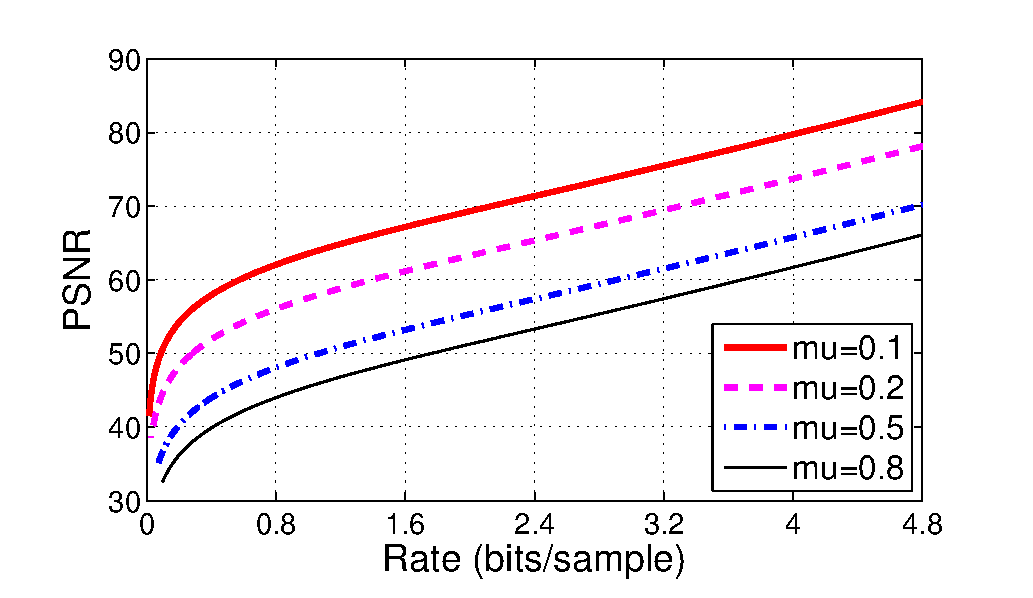
\includegraphics[width = 0.5\linewidth]{Figures/section3/RD_Cauchy_z=0_75_p=0} &
\includegraphics[width = 0.5\linewidth]{Figures/section3/RD_Cauchy_z=1_p=0_5} \\
{\small (a) $z=3/4,\;f=0$} & {\small (b) $z=1,\;f=1/2$} \\
\includegraphics[width = 0.5\linewidth]{Figures/section3/RDDerivative_Cauchy_z=0_75_p=0} &
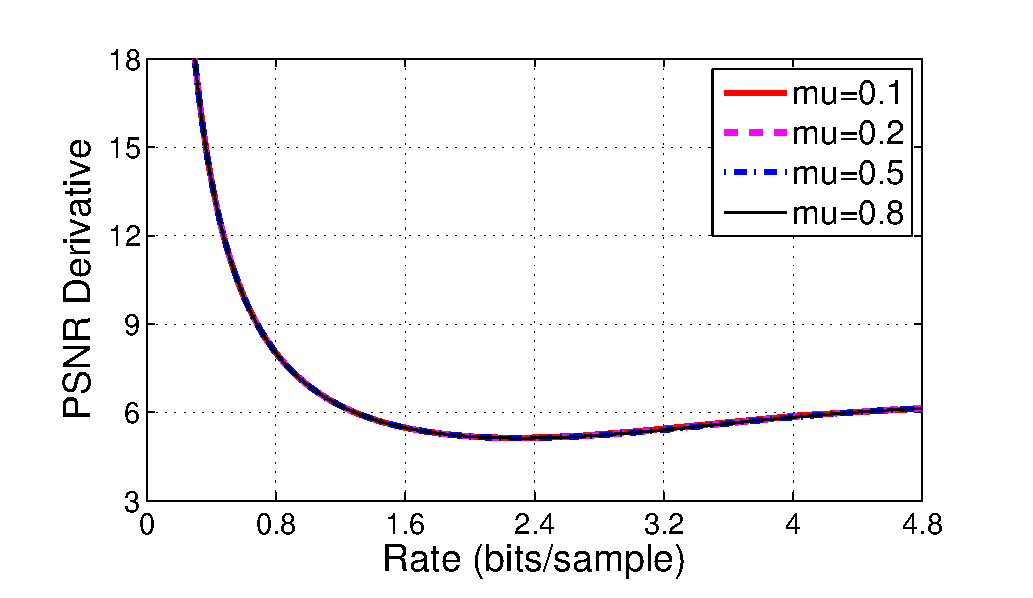
\includegraphics[width = 0.5\linewidth]{Figures/section3/RDDerivative_Cauchy_z=1_p=0_5} \\
{\small (c) $z=3/4,\;f=0$} & {\small (d) $z=1,\;f=1/2$}
\end{tabular}
\end{center}
\vspace{-20pt}
\caption{\label{fig:RD_mu}
Curves of PSNR-R function and its derivative for different $\mu$ of Cauchy distribution under DZ+UTQ/NURQ (two quantizer configurations are used).}
\end{figure*}


\section{Universal Principles of Quantizer Design for Various Sources}
\label{sec:principle}

The necessary conditions for a scalar quantizer to achieve optimum R-D performance (i.e., minimizes the average distortion with entropy constraint) were formulated in \cite{Farvardin_TIT1984}. Specifically, under MSE criterion, Max \cite{Max_TIT1960} obtained the famous condition that, for each quantization index $k$, the reconstruction value $R_k$ should be located at the \emph{centroid} of the area of PDF $p(x)$ within quantization interval $I_k$. Thus, for the symmetric DZ+UTQ/NURQ scheme, the optimum design requires:
\begin{equation}\label{equ:formula-OptQuant}
	{R_k}^* = \int_{(k-1+z)s}^{(k+z)s} xp(x)dx / \int_{(k-1+z)s}^{(k+z)s} p(x)dx, \quad k \ge 1.
\end{equation}
Due to the symmetry, we only consider the positive half without loss of generality.

Based on (\ref{equ:formula-OptQuant}), we now deduce the necessary constraint on $z$ and $f$ for DZ+UTQ/NURQ design to achieve optimum R-D performance. Note that we assume nothing special about the source, except that it's zero-mean and the PDF $p(x)$ is monotonically non-increasing in positive x-axis, which is true for all source distributions of interest.

First of all, the reconstruction value $R_k$ needs to be located within the quantization interval $I_k$ (the prerequisite of being located at the \emph{centroid}). Then with (\ref{equ:interval}) and (\ref{equ:DZ+UTQ/NURQ}), the preliminary constraint on $z$ and $f$ can be obtained:
\begin{equation}\label{equ:formula-PreConstraint}
	 T_k \le R_k < T_{k+1} \Rightarrow (k-1+z)s \le (k+f)s < (k+z)s \Rightarrow 0 < z - f \le1.
\end{equation}

Next, we further refine this constraint using (\ref{equ:formula-OptQuant}). Given that $p(x)$ is monotonically non-increasing in positive x-axis, and $p(x) > 0$, for $0 < a < b$, it can be proved that (a proof is provided in the Appendix):
\begin{equation}\label{equ:formula-Inequity}
	\int_a^b xp(x)dx \le \frac{a+b}{2} \int_a^b p(x)dx.
\end{equation}
Let $a=(k-1+z)s$, $b=(k+z)s$. Then (\ref{equ:formula-Inequity}) becomes:
\begin{equation}\label{equ:formula-Inequity1}
	\int_{(k-1+z)s}^{(k+z)s} xp(x)dx \le (k+z-\frac{1}{2}) s \int_{(k-1+z)s}^{(k+z)s} p(x)dx, \quad k \ge 1.
\end{equation}
By integrating (\ref{equ:formula-OptQuant}) and (\ref{equ:formula-Inequity1}), we obtain that:
\begin{equation}\label{equ:formula-Inequity2}
	{R_k}^* \le (k+z-\frac{1}{2})s, \quad k \ge 1.
\end{equation}
From (\ref{equ:DZ+UTQ/NURQ}) and (\ref{equ:formula-Inequity2}), we know that the optimum quantizer design requires $(k+f)s \le (k+z-\frac{1}{2})s$, which is $z-f \ge \frac{1}{2}$. Thus the preliminary constraint (\ref{equ:formula-PreConstraint}) can be refined to $\frac{1}{2} \le z-f \le 1$, also written as:
\begin{equation}\label{equ:formula-RefConstraint}
	z = f+d, \quad \frac{1}{2} \le d \le 1,
\end{equation}
which is the necessary constraint for DZ+UTQ/NURQ design to be optimum.

Derived without a specific $p(x)$(PDF) formula, this design principle is universal to all commonly-used distributions and should apply to various sources. In \cite{Sullivan_VCIP2005}, the DZ+UTQ/NURQ quantizer's performance for Laplacian and Gaussian source is theoretically analyzed, and the results about the optimum values of quantizer parameters are completely consistent with this principle. As further validation, we present simulation experiments for Cauchy distribution, which still lacks thorough analysis in the literature. For Cauchy distribution with $\mu = 0.2$ and $0.8$, R-D performance comparison of different $z-f$ values for DZ+UTQ/NURQ is exhibited in Fig. \ref{fig:RD_different_patterns}, which clearly demonstrates the superiority of those values satisfying (\ref{equ:formula-RefConstraint}).

\begin{figure*}
\begin{center}
\begin{tabular}{cc}
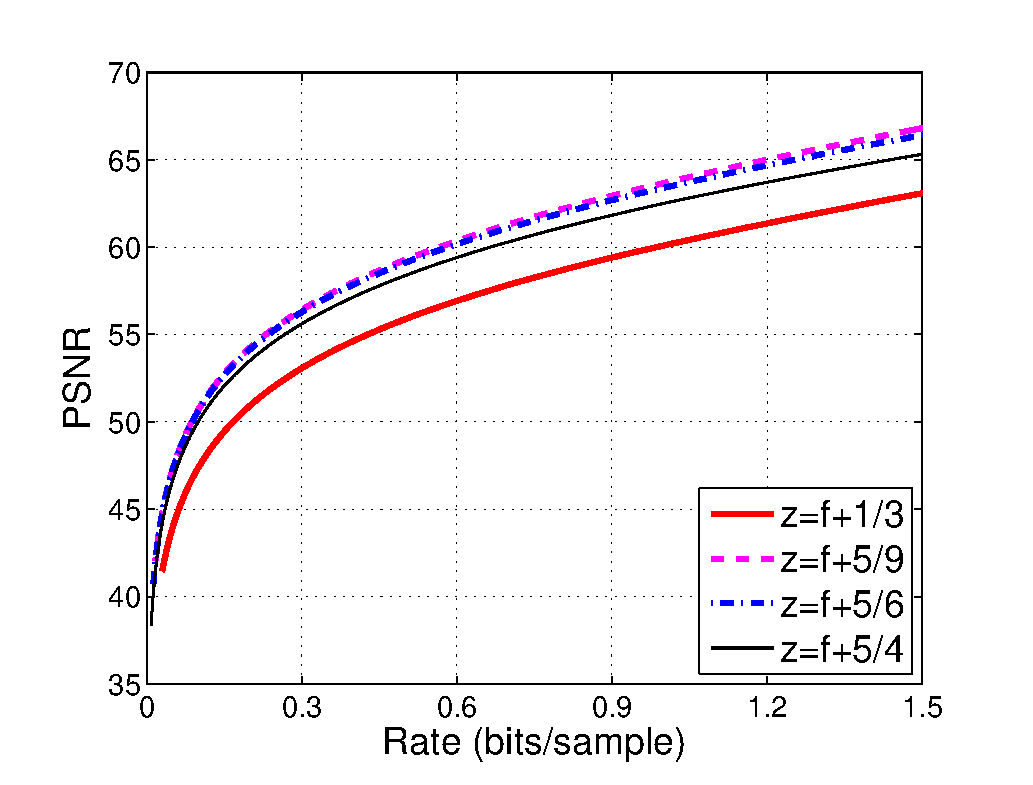
\includegraphics[width = 0.45\linewidth]{Figures/section4/RD_Cauchy_mu=0_2_linear_patterns} &
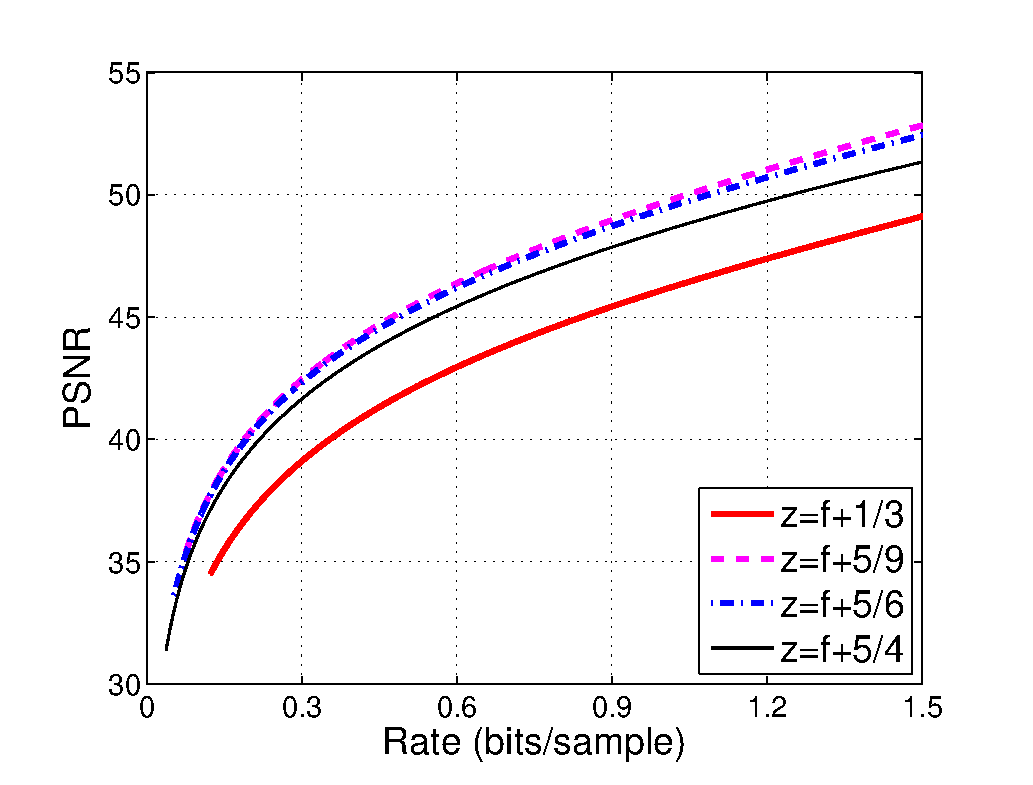
\includegraphics[width = 0.45\linewidth]{Figures/section4/RD_Cauchy_mu=0_8_linear_patterns} \\
{\small (a) Cauchy $\mu=0.2$} & {\small (b) Cauchy $\mu=0.8$}
\end{tabular}
\end{center}
\vspace{-20pt}
\caption{\label{fig:RD_different_patterns}
R-D performance comparison of different $z-f$ values for DZ+UTQ/NURQ.}
\end{figure*}

Guided by this universal principle, when selecting parameters of DZ+UTQ/NURQ for any source, one should first of all ensure that $z-f=d$ satisfies (\ref{equ:formula-RefConstraint}). Then for some particular sources, we continue to show that, the value $z-f$ can actually be used as a precise classifier for the quantizer performance.

Consider the quantization interval $I_k$ ($k \ge 1$), where the reconstruction value $R_k$ divides it into two parts: $\overline{T_k R_k}$ and $\overline{R_k T_{k+1}}$. For some ``broad-tailed" or ``fat-tailed"$^1$\footnote{$^1$ https://en.wikipedia.org/wiki/Fat-tailed\_distribution} distributions, e.g., some members of the Cauchy family \cite{Farvardin_TIT1984}, in quantization intervals other than the dead-zone, the PDF can be precisely approximated with a straight line. For a straight line PDF, whether $R_k$ is at the centroid of the area in $I_k$, or equivalently, whether the quantizer has optimum performance, would be determined exclusively by the ratio $\overline{T_k R_k} / \overline{R_k T_{k+1}}$, which therefore can serve as a measurement for the performance of the quantizer. In other words, if two DZ+UTQ/NURQ designs ($z_1, f_1$) and ($z_2, f_2$) result in the same value of $\overline{T_k R_k} / \overline{R_k T_{k+1}}$, their R-D performance would also be identical. According to (\ref{equ:DZ+UTQ/NURQ}), the $\overline{T_k R_k} / \overline{R_k T_{k+1}}$ values of the two quantizers being the same implies that:
\begin{equation}\label{equ:formula-ratio}
\frac{(k+f_1)-(k-1+z_1)}{(k+z_1)-(k+f_1)} = \frac{(k+f_2)-(k-1+z_2)}{(k+z_2)-(k+f_2)},
\end{equation}
which can be reduced to $z_1 - f_1 = z_2 - f_2$. Reasoning back, we can obtain that: for two quantizer designs ($z_1, f_1$) and ($z_2, f_2$), the performance of them will be the same as long as $z_1 - f_1 = z_2 - f_2$, regardless of the specific values of these parameters.

Although not as universal as the previous one, this principle still applies to a large class of sources with ``broad-tailed" distributions. Simulation validation for Cauchy distribution with $\mu = 0.5$ is provided in Fig. \ref{fig:RD_same_pattern}, where R-D performance comparison of different DZ+UTQ/NURQ designs with the identical $z-f$ value is shown. It is observed that, for the same $z-f$ value, all the PSNR-R curves are overlapped, indicating the same R-D performance regardless of the specific $z$, $f$ values.

\begin{figure*}
\begin{center}
\begin{tabular}{cc}
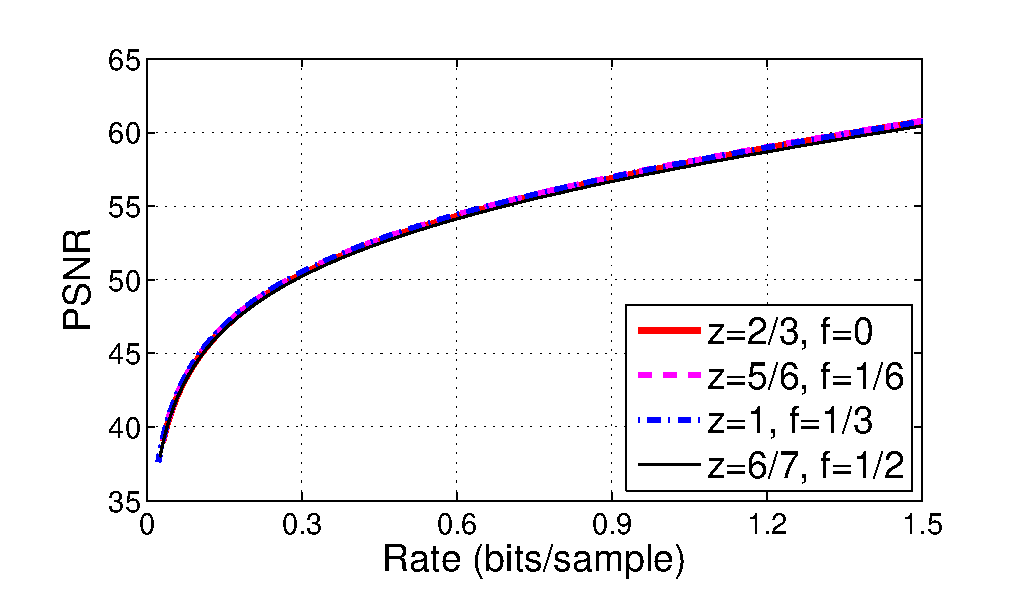
\includegraphics[width = 0.45\linewidth]{Figures/section4/RD_Cauchy_mu=0_5_z=p+0_67} &
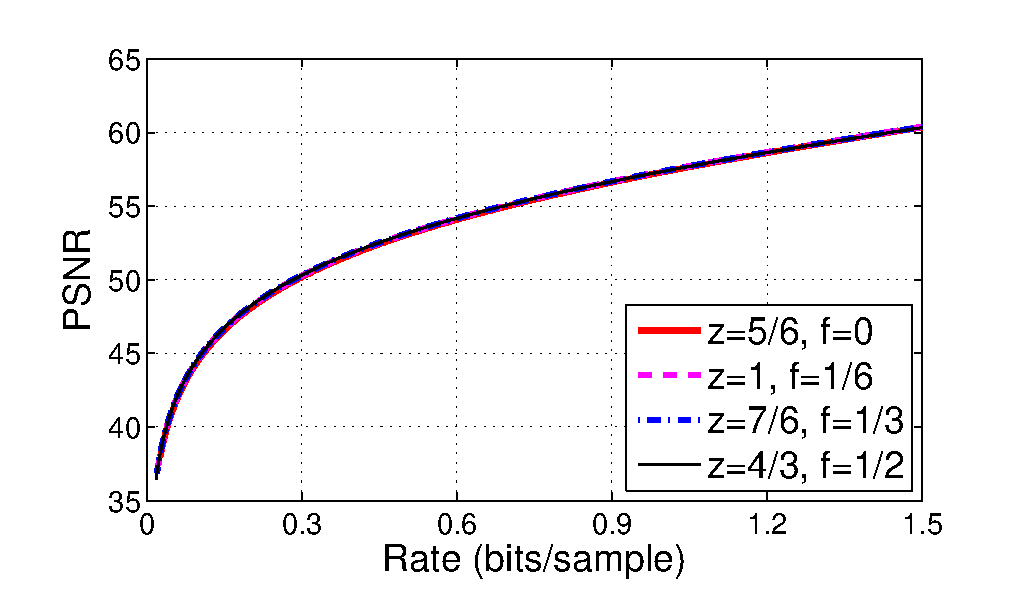
\includegraphics[width = 0.45\linewidth]{Figures/section4/RD_Cauchy_mu=0_5_z=p+0_83} \\
{\small (a) $z=f+2/3$} & {\small (b) $z=f+5/6$}
\end{tabular}
\end{center}
\vspace{-20pt}
\caption{\label{fig:RD_same_pattern}
R-D performance comparison of different quantizer designs with identical $z-f$ value for Cauchy $\mu=0.5$.}
\end{figure*}

In summary, the two principles provide a convenient way to simplify R-D performance analysis and guide the practical quantizer design for various source distributions. Benefiting from them, the reason why the DZ+UTQ/NURQ designs applied in video/image coding standards (e.g. in H.264/AVC, $z$ is set to $2/3$ in intra coding and $5/6$ in inter coding, $f$ is set to $0$ \cite{Sullivan_VCIP2005}) are effective can now be clearly seen.

\section{Conclusion}
\label{sec:conclusion}

In this paper, universal property and principles that apply to various source distributions are revealed and validated. First, for any source distribution composed of a scaling factor and the remaining part, the scaling factor does not affect the derivative of its R-D function (with PSNR as distortion criteria). Second, for the DZ+UTQ/NURQ scheme to achieve optimum R-D performance, its parameters should satisfy the necessary constraint of $\frac{1}{2} \le z - f \le 1$, and the value of $z - f$ is also a precise performance classifier for source distributions of particular forms. These results can provide insights and assistance in R-D modeling and quantizer design for real coding applications, where the source distribution may be complex and uncertain.

\section*{Appendix}
\label{sec:appendix}

In this appendix, we prove: $\int_a^b xp(x)dx \le \frac{a+b}{2} \int_a^b p(x)dx$, given that $p(x)$ is monotonically non-increasing in positive x-axis, $p(x) > 0$, and $0 < a < b$.

Let $F(t) = \int_a^t xp(x)dx - \frac{a+t}{2} \int_a^t p(x)dx, t \in [a, b]$. Then $F^{\prime}(t) = tp(t) - [\frac{1}{2}\int_a^t p(x)dx + \frac{a+t}{2}p(t)] = \frac{t-a}{2}p(t) - \frac{1}{2}\int_a^t p(x)dx = \frac{1}{2}\int_a^t p(t)-p(x)dx $. Since $p(x)$ is monotonically non-increasing, for $x \in [a, t]$ we have $p(t) \le p(x)$, which implies $F^{\prime}(t) \le 0$. Therefore $F(t)$ is also monotonically non-increasing. Then with $b > a$, we obtain $F(b) \le F(a)$, which is $\int_a^b xp(x)dx - \frac{a+b}{2} \int_a^b p(x)dx \le 0$, i.e., $\int_a^b xp(x)dx \le \frac{a+b}{2} \int_a^b p(x)dx$. $\square$

% It's prettier with more space.
\iffalse
\begin{eqnarray*}
F^{\prime}(t) &=& tp(t) - [\frac{1}{2}\int_a^t p(x)dx + \frac{a+t}{2}p(t)]\\&=& \frac{t-a}{2}p(t) - \frac{1}{2}\int_a^t p(x)dx \\&=& \frac{1}{2}\int_a^t p(t)-p(x)dx
\end{eqnarray*}
\fi

\section*{References}
\bibliographystyle{IEEEtran}
\bibliography{refs}

\end{document}
